\chapter{Results}
\label{chap:results}
\section{Line Feature Sampling Inacurracy}
\label{sec:linefeature_inaccuracy}
The faces in the set of given scans all contain large holes in the regions of the eyes and the ears. Some also have holes on top of the nose.
Due to this circumstance the vertices with the most similar directions to that of the sample point are farther away a suboptimal location. 
Consequently, the projected sample points of the line features may be off target in cases where the holes are very large. In effect, the projected line is distorted, as can be seen in \ref{fig:linefeature_comparison} on the right side. 
\begin{figure}[h!]
    \centering
    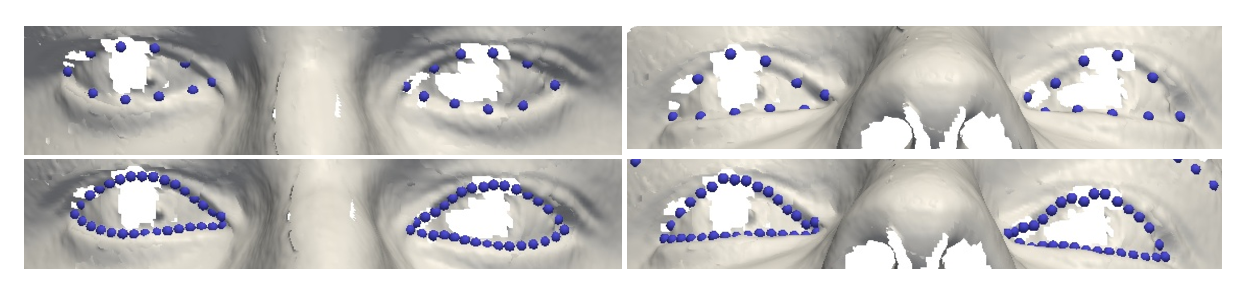
\includegraphics[width=\textwidth]{./resources/img/linefeatures_eyes.pdf}
    \caption{Line Features}
    \label{fig:linefeature_comparison}
\end{figure}
On the different data sets quality of the projected line features varies significantly, because each scan has different holes. If a scan contains large holes one can say overall that the distortion of a projected line features increases with the amount of sampled points. 
On different data sets the performance of the projection of the line features for a large number of
samples, i.e. 30, varied significantly. 
An easy workaround to this problem is to reduce the amount of sampled points. By using only 5-10 sample points per curve most datasets rendered near perfect results. 
However, when the holes are too large this workaround also fails, slight distortions can be made out in \ref{fig:linefeature_comparison} top right.
If the distortions are not too big they are accounted for by the additive Gaussian Noise in the joint distribution \ref{sec:noisemodel}.
However, as long as the method is dependent on the data from the scans - the size of the holes in the meshs - it lacks generality and generality is exactly the basis for feasible and reproducable registration results.\\

\section{The effect of Line Features}
In this section we illustrate the effect of the line features on the registration results.
For this purpose we compare the feature regions of registered templates with and without line features with the respective target. We use up-close images of the various feature regions for a qualitative comparison.
Target with mean texture projected on to it.
\begin{figure}[h!]
    \centering
    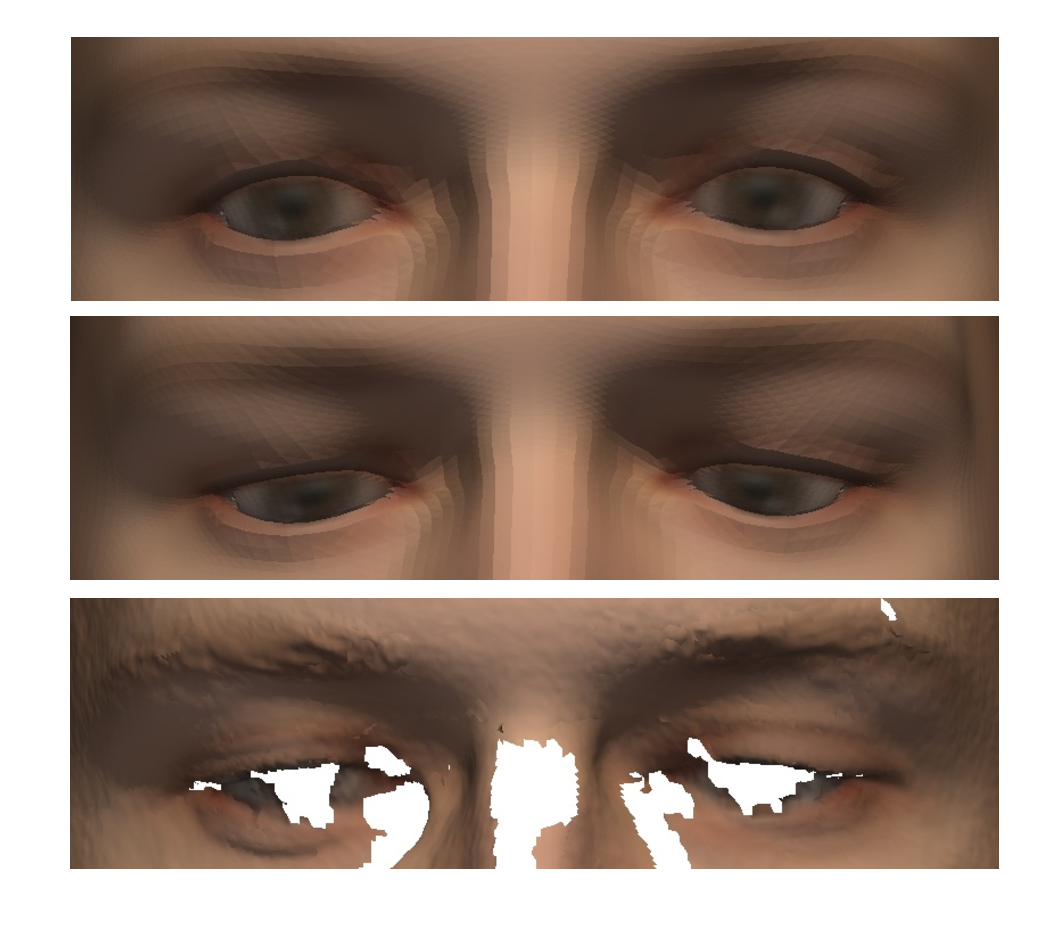
\includegraphics[width=.9\textwidth]{./resources/img/00029_eyes_comparison.pdf}
\caption{A comparison of the fitting results concerning the eyes. The first image displays the eyes in the registered template without line features. The second image has been registered with line features. As one can see the eyes in the top image are in the right position, because the displacement of the corners is defined by the given landmarks. However, compared to the middle image the contours of the eyes are very different. The incorporation of line features in the middle
image has lead to a much better correspondence with the eyes of the target mesh, displayed at the bottom.}
\label{fig:fiteyes}
% reference in text by \ref{$figure-name}
\end{figure}

\begin{figure}[h!]
    \centering
    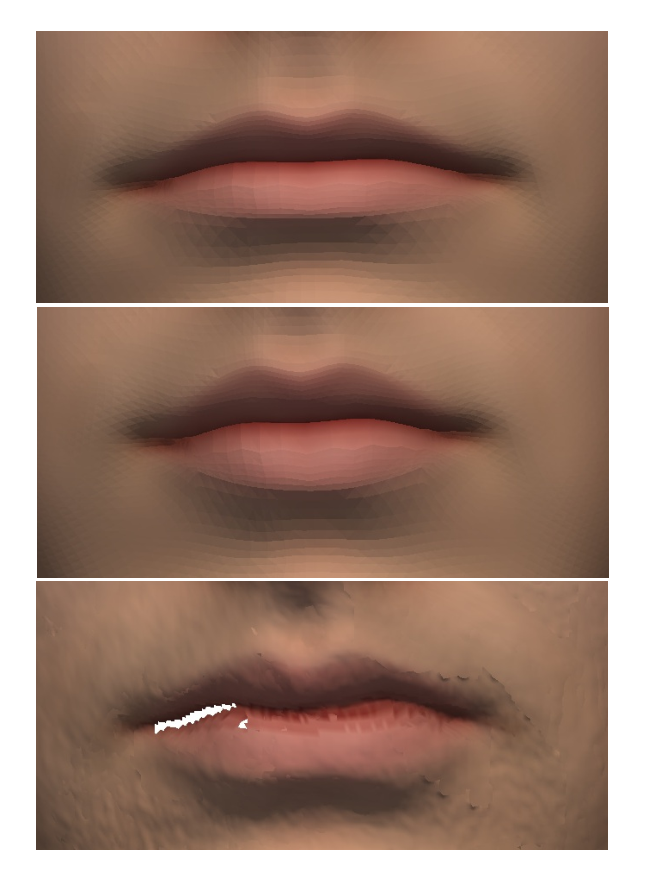
\includegraphics[width=.8\textwidth]{./resources/img/00029_mouth_comparison.pdf}
    \label{fig:00029_mouth_comparison}
    \caption{At the top again is the mouth fitted without line features and beneath the one with line features. The lips in the top image are considerably thinner although the position of the mouth is of course correct due to the displacement of the landmarks in marked at the corners of the mouth. The lips in the middle image are fuller an match the mouth of the target better in this respect. However, the lower lip of the target appears to be bimodal while the lip of the fit is still unimodal as in the template mesh.}
\end{figure}
\pagebreak

\begin{figure}[h!]
    \centering
    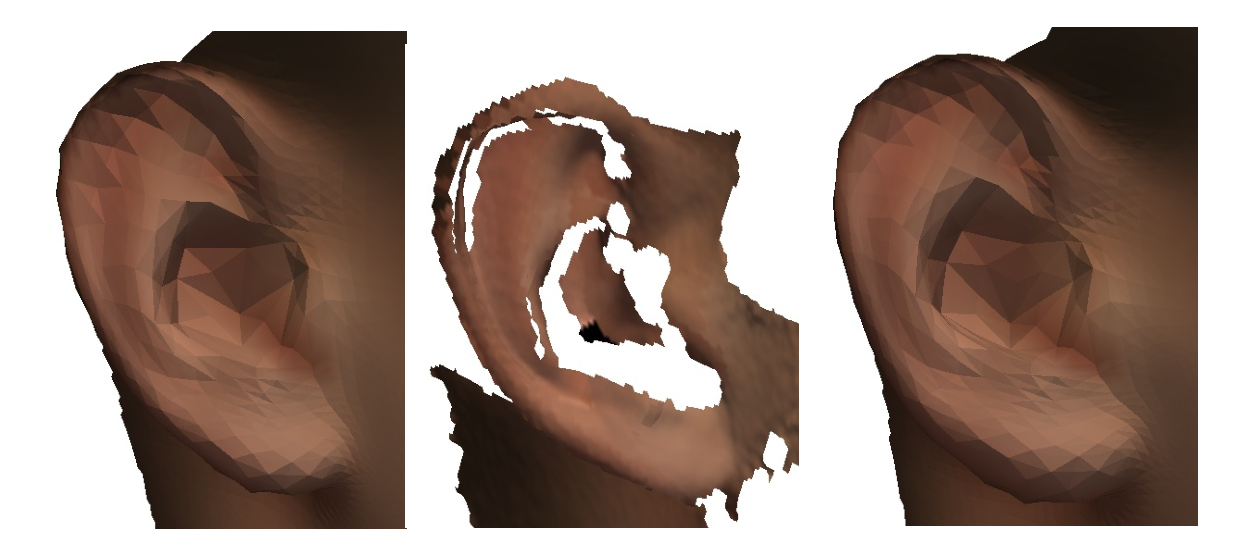
\includegraphics[width=\textwidth]{./resources/img/00029_left_ear_comparison.pdf}
\caption{Ears}
\label{fig:fitears}
\caption{A comparison of the fitting results of the ears. The image on the left hand side is the fit without line features and image on the right hand side is the fit using line features. The target is displayed between the two. The ear on the left is narrower than the ear of the target and the ear of the fit using line features.}
% reference in text by \ref{$figure-name}
\end{figure}

\subsection{Visualized Distance}
A further way to evaluate the matching of the contour lines is to analyse distance maps. These are obtained by taking the differences of the nearest points in the deformed template and the target mesh.
Distance maps to show distance for semantic correspondences

\begin{figure}[h!]
    \centering
    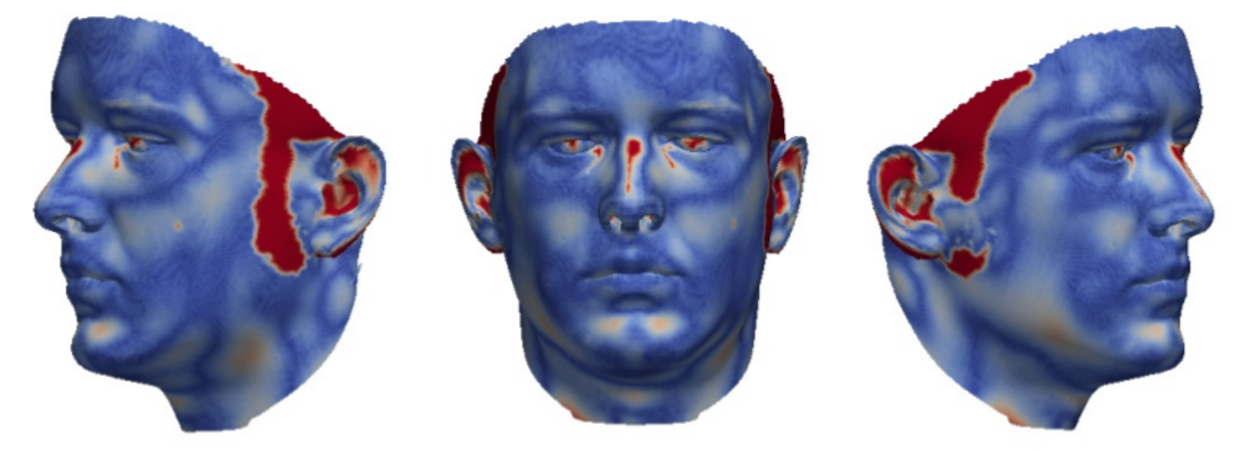
\includegraphics[width=.8\textwidth]{./resources/img/00029_distmap.pdf}
    \label{fig:00029distmap}
    \caption{Distance face of fit displayed in fig. \ref{fig:fitcomparison}} in range [0, 3mm]. Except for the holes in the target mesh all vertices in the template have less than 3mm distance to their nearest neighbours on the target mesh. The distance map doesn't show semantical correspondence.}
% reference in text by \ref{$figure-name}
\end{figure}
\begin{figure}[h!]
    \centering
    \subfloat[target mesh with projected template texture]{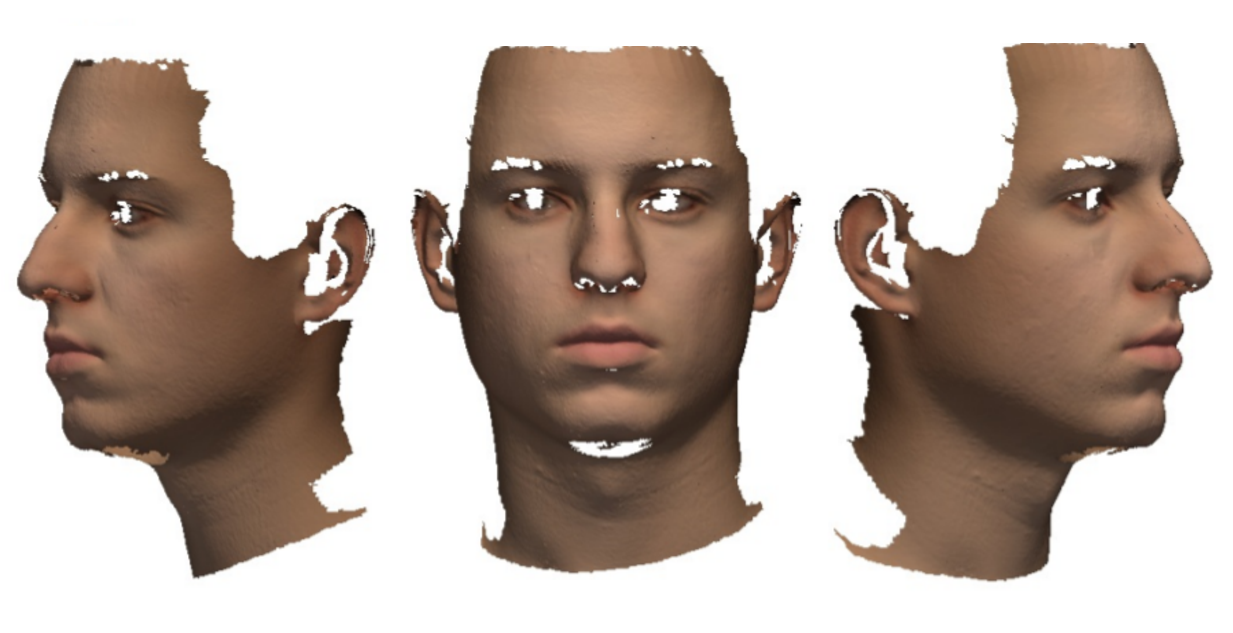
\includegraphics[width=\textwidth]{./resources/img/00303_textured_target.pdf}}\\
    \subfloat[deformed template fitted to the target]{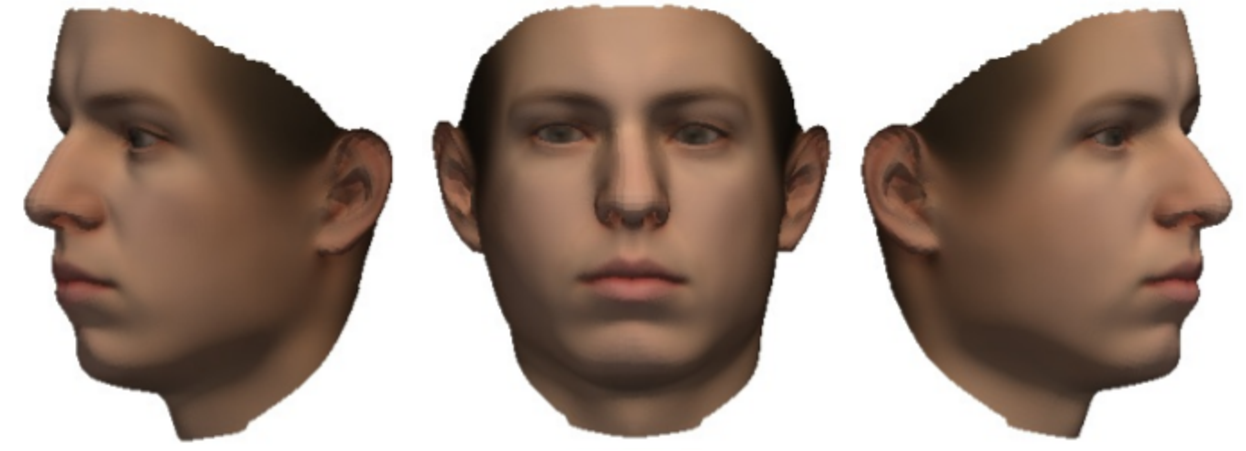
\includegraphics[width=\textwidth]{./resources/img/00303_fit.pdf}}\\
    \subfloat[distance map]{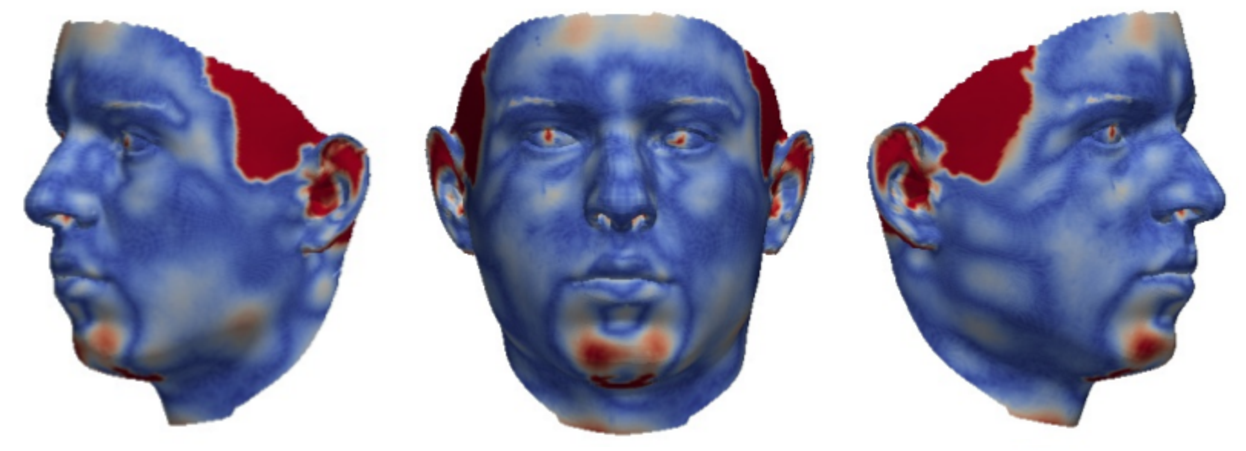
\includegraphics[width=\textwidth]{./resources/img/00303_distmap.pdf}}
    \caption{This figure shows the fit of the template mesh to a different target face and the distance map in a range of 0-3 millimeters.}
\label{fig:00303distmap}
% reference in text by \ref{$figure-name}
\end{figure}

\begin{figure}[h!]
    \centering
    \subfloat[Distance image of the mouth of fit in \ref{fig:00029fit}]{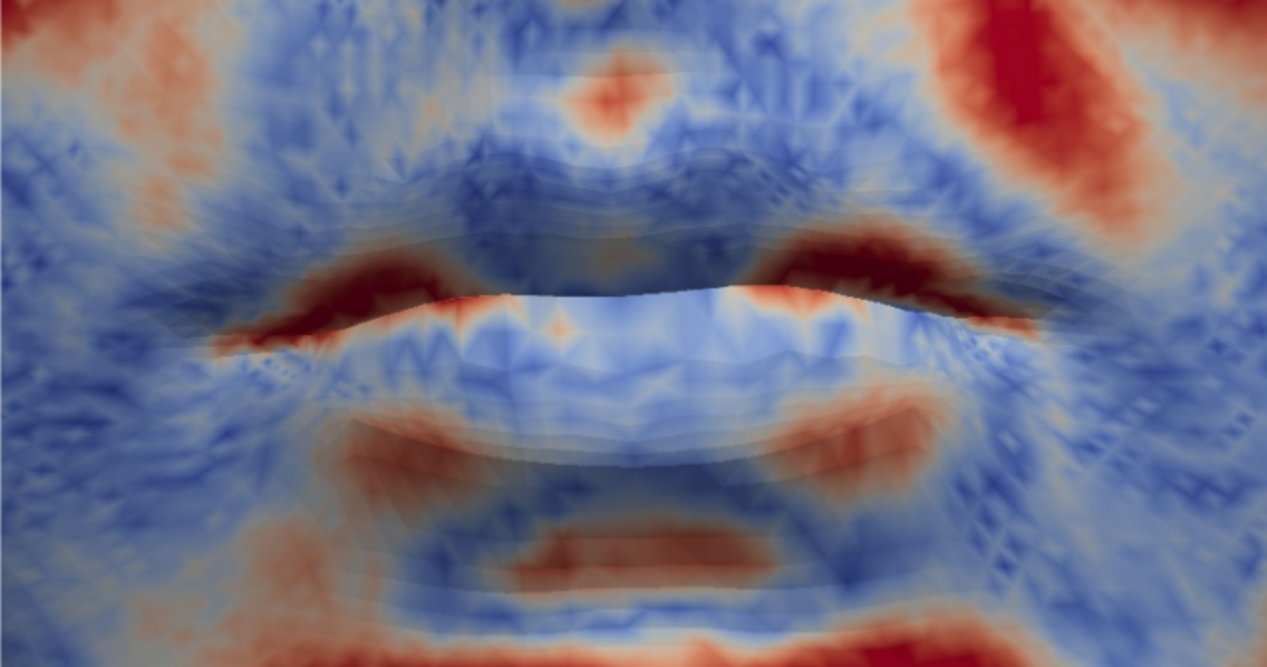
\includegraphics[width=.5\textwidth]{./resources/img/00029_dist_mouth_0_1_cropped.pdf}}
    \subfloat[Distance image of the mouth of fit in \ref{fig:00303fit}]{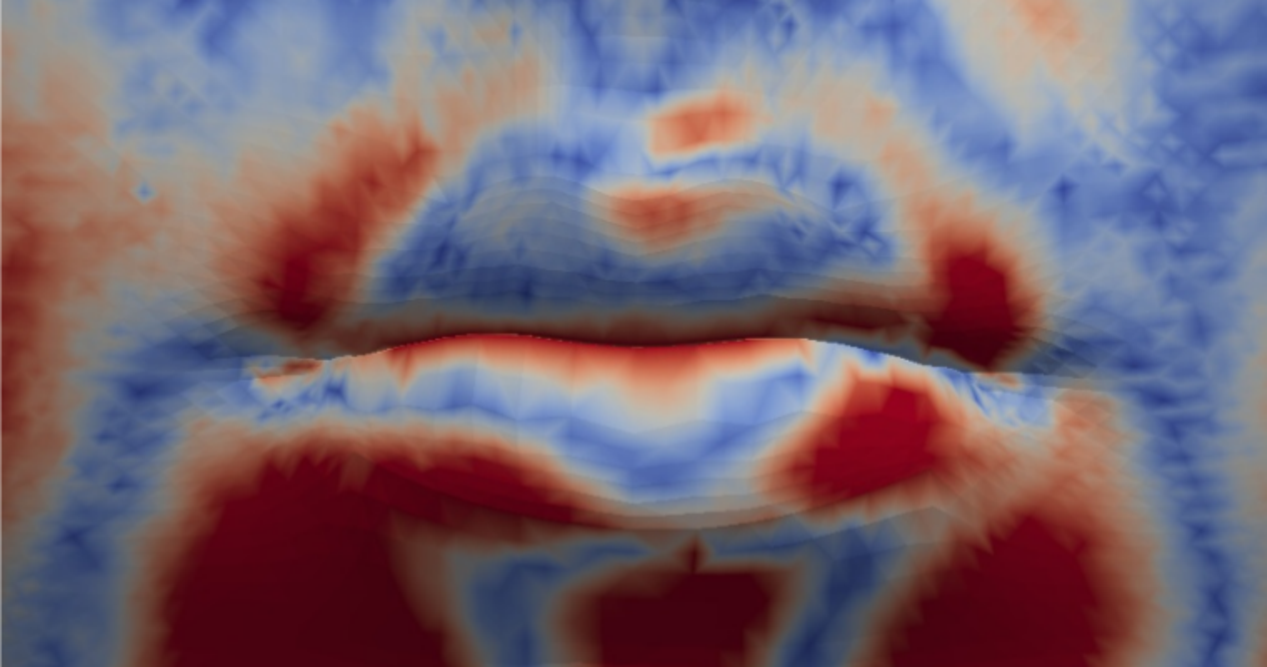
\includegraphics[width=.5\textwidth]{./resources/img/00303_dist_mouth_0_1_cropped.pdf}}
    \label{fig:distmaplips}
    \caption{Both distance images are on a scale of 0-1mm [blue, red]. The fit of the lips is better in a) where the area along the contour lines of the lips is mostly light blue. In b), however, the distances in the region of the lips often exceeds 1mm and quality of the fit is not as good.}
\end{figure}

\begin{figure}[h!]
    \centering
    \subfloat[00029 eyes distance]{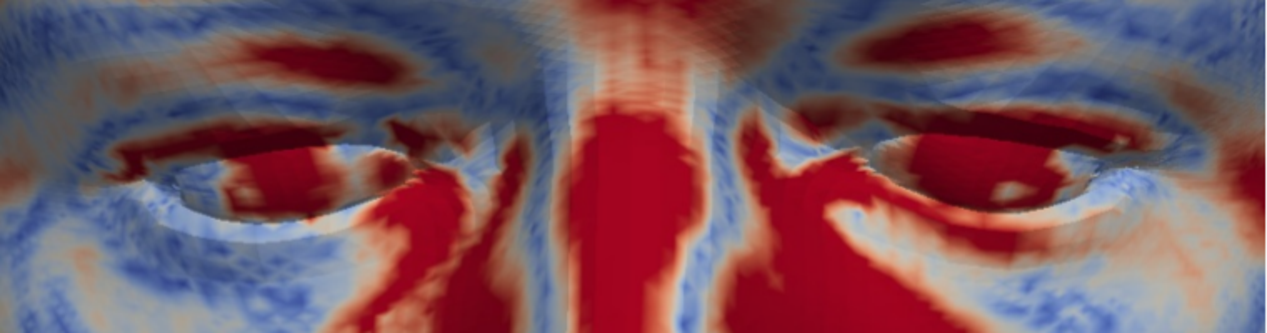
\includegraphics[width=.8\textwidth]{./resources/img/00029_dist_eyes_0_1_cropped.pdf}}\\
    \subfloat[00303 eyes distance]{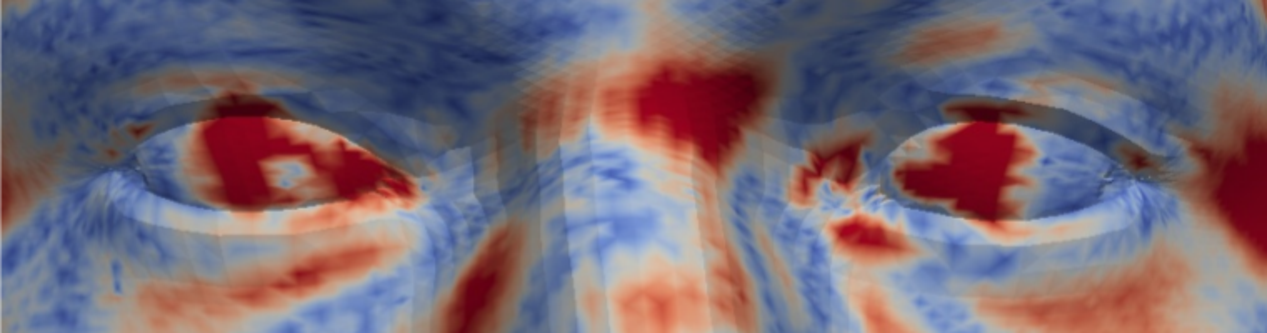
\includegraphics[width=.8\textwidth]{./resources/img/00303_dist_eyes_0_1_cropped.pdf}}
    \label{fig:distmapeyes}
    \caption{Again both distance images are shown on a scale of 0-1mm [blue, red]. The fit in a) has a lot red areas, because the target mesh has large holes in the region of the eyes and along both sides of the nose and on top of the nose. The bottom inner contour of the left eye is however matched very well. The same can be said for b). Here, the bottom inner contour of the right eye is also mathed fairly well.}
\end{figure}

\subsection{Caricatures}
Caricatures of the deformed template are another way of inspecting the quality of the registration results. Points in the same feature regions should be displaced in a very similar manner. Therefore, by adding the deformation field to the target multiplied by a scaling parameter exceeding 1, these regions should ideally become more prominent in the resulting mesh. The same rule applies to distortions/artifacts which also become more visible with an increase in the scaling factor.

\begin{figure}[h!]
    \centering
    %\subfloat[fit]{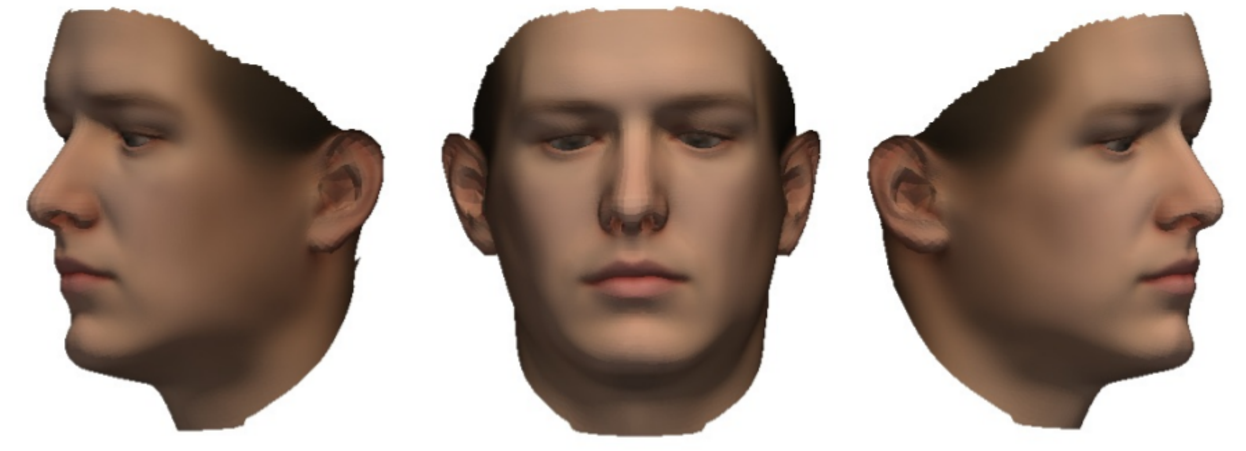
\includegraphics[width=\textwidth]{./resources/img/00029_fit.pdf}}\\
    \subfloat[scaling factor 1.3]{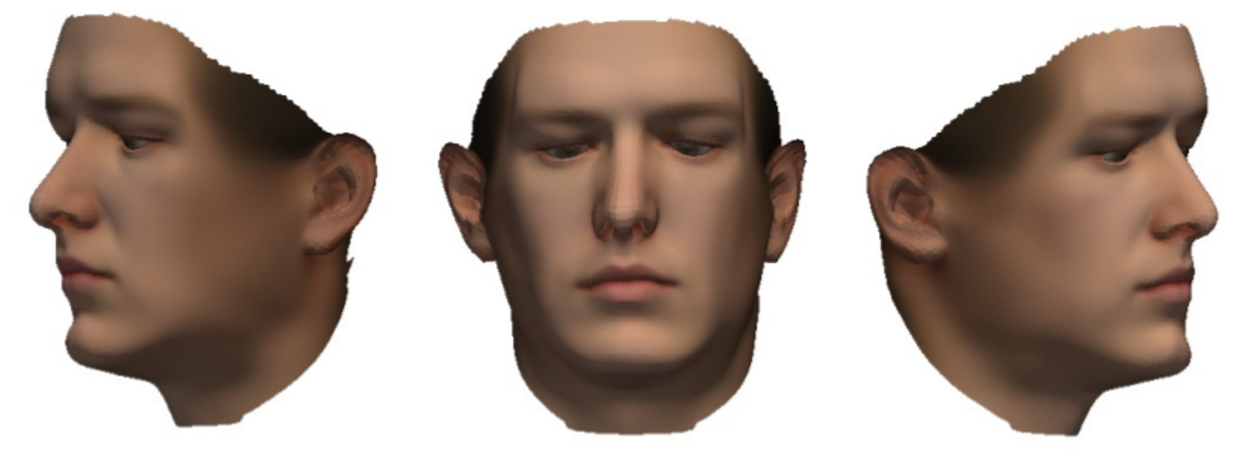
\includegraphics[width=.9\textwidth]{./resources/img/00029_caricature_1_3.pdf}}\\
    \subfloat[scaling factor 1.6]{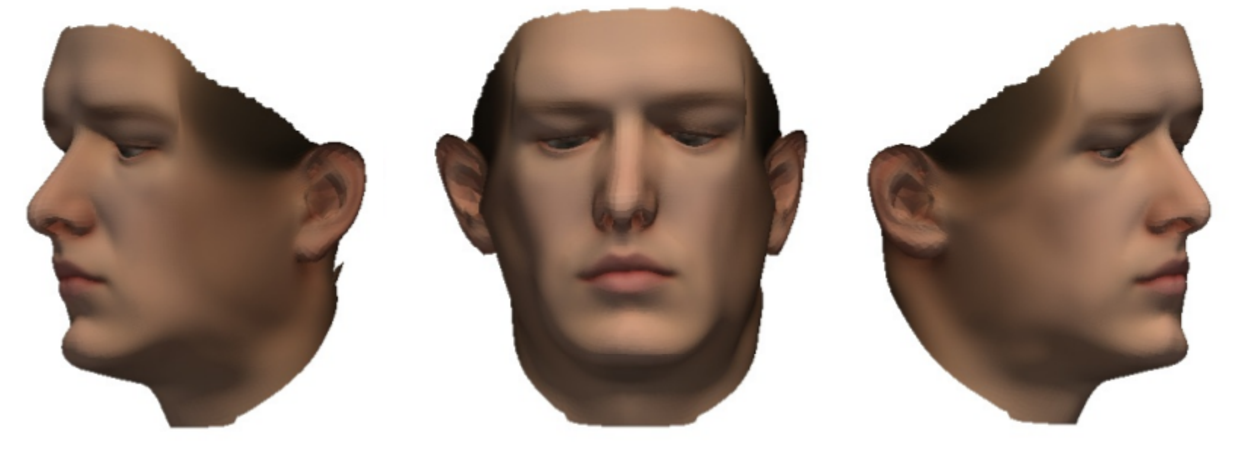
\includegraphics[width=.9\textwidth]{./resources/img/00029_caricature_1_6.pdf}}\\
    \subfloat[scaling factor 2]{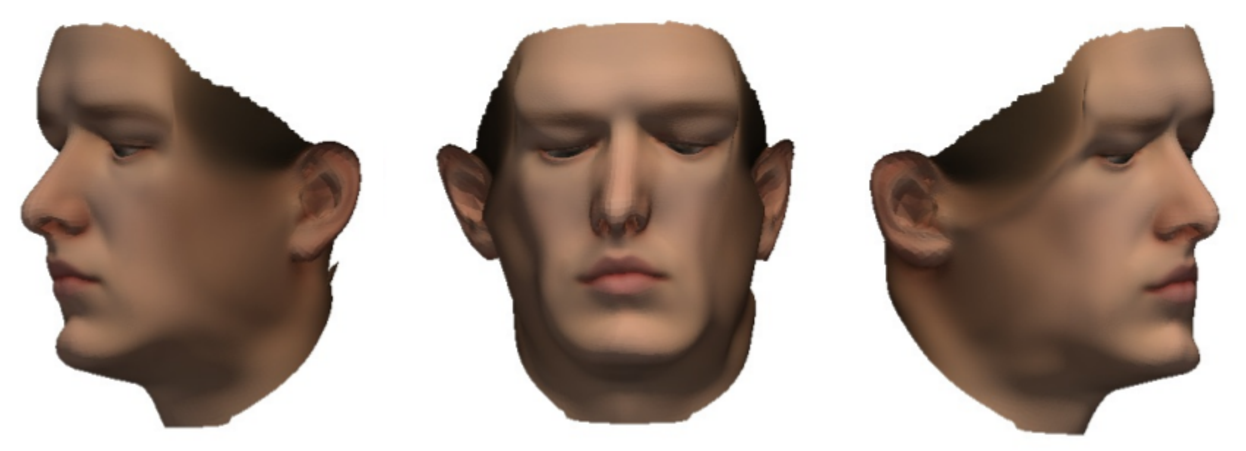
\includegraphics[width=.9\textwidth]{./resources/img/00029_caricature_2.pdf}}\\
    \caption{Caricatures of the fit in fig. \ref{fig:00029fit} with different parameter values. With an increasing scaling factor the face is twisted more to the left, with the mouth and the nose while the ears become pointier. The eyelids are shut more and more with each step. Also a fold begins developing to both sides of the head. This artifact is cause by the increase of the minimal displacements of the template mesh vertices which have no corresponding vertices on the target
mesh and are not completely ignored by the Tukey estimator.}
\label{fig:00029_caricature}
% reference in text by \ref{$figure-name}
\end{figure}

\begin{figure}[h!]
    \centering
    \subfloat[scaling factor 1.3]{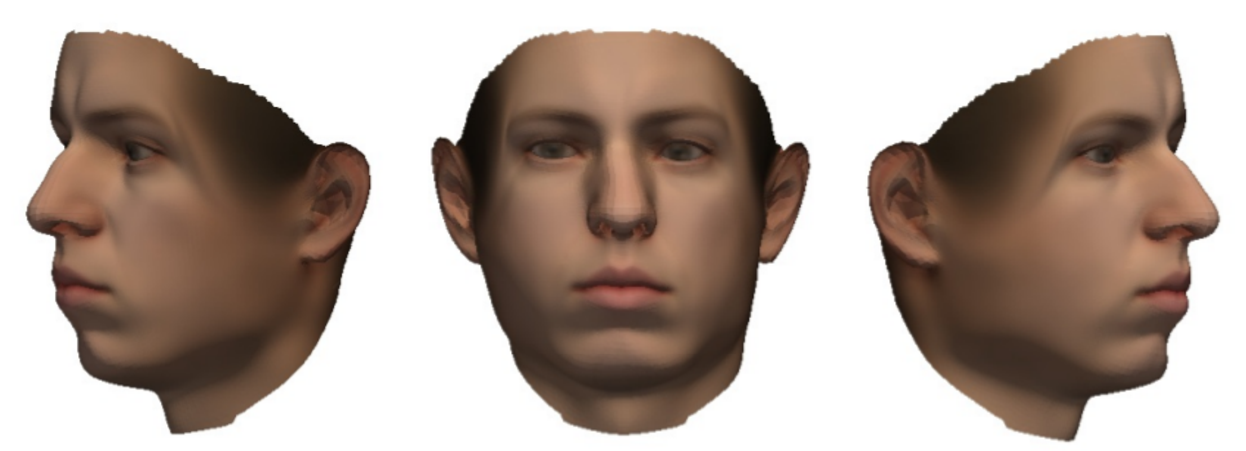
\includegraphics[width=.9\textwidth]{./resources/img/00303_caricature_1_3.pdf}}\\
    \subfloat[scaling factor 1.6]{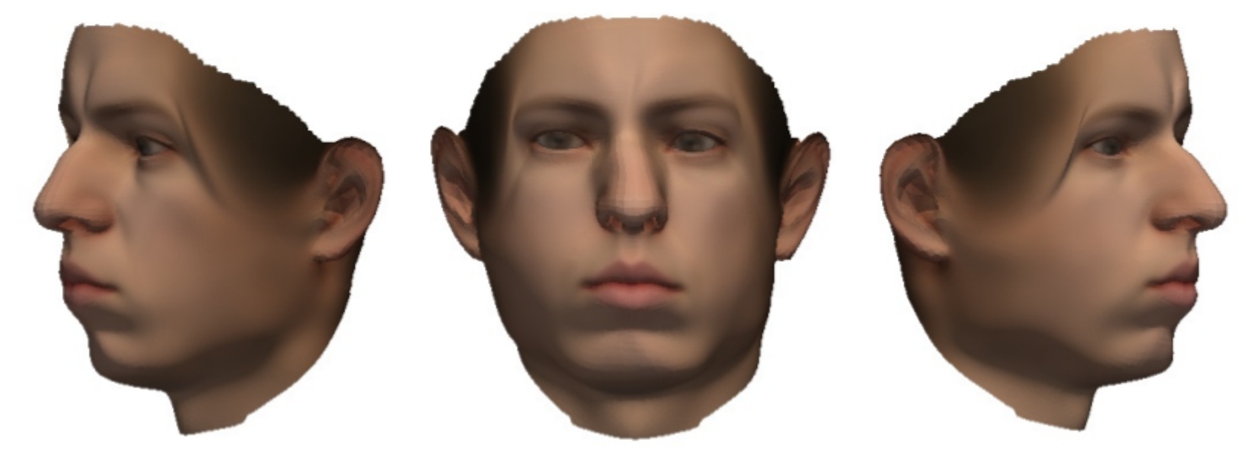
\includegraphics[width=.9\textwidth]{./resources/img/00303_caricature_1_6.pdf}}\\
    \subfloat[scaling factor 2]{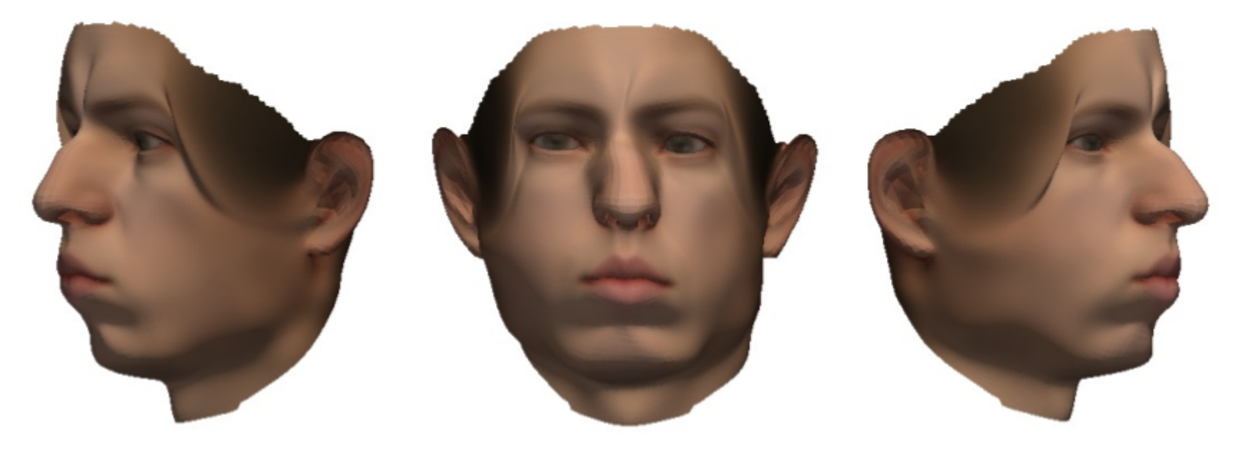
\includegraphics[width=.9\textwidth]{./resources/img/00303_caricature_2.pdf}}
    \caption{Caricatures of fit in \ref{fig:00303fit} for three different scaling factors. Here, the exageration of a slightly hooked nose can be observed. In this case the face is bent slightly to the right and lips are pressed together and foreward. The folds on both sides of the head are prominent than in the other example.} 
\label{fig:00303_caricature}
% reference in text by \ref{$figure-name}
\end{figure}

\begin{comment}
\subsection{Effects of the Covariance Function}
A Gaussian Kernel
00125 - scan of old man --> wrinkles can't be modelled through this smooth definition of covariance - adjust covariance function
\end{comment}

